\chapter{微分方程速成}\label{app:de}

微分方程 (DE) 是动态系统建模的基本工具，可大致分为 \emph{ 常微分方程 } (ODE)、\emph{ 随机微分方程 } (SDE) 和 \emph{偏微分方程}（PDE）。

ODE 描述了系统的状态如何根据精确的规则随时间变化，因此知道起点就可以准确地确定未来的路径。 SDE 为这种演化增加了随机性，对噪声或不确定性如何影响系统行为进行建模，使结果具有概率性而非固定性。偏微分方程解释了取决于时间和空间等多个变量的函数如何一起演化，捕获热扩散、波移动等现象，或 \emph{ 随机系统中概率密度的时间演化}（如福克尔-普朗克方程）。这些类型的微分方程形成了一种基本语言，用于理解系统在确定性和随机影响下如何随时间和空间演化。

在本章中，我们提供微分方程的基本先决条件。

\chapterlearning{
  \item 通过速度场、解轨迹以及存在性和唯一性的作用来解释 ODE；

  \item 使用积分因子来揭示半线性 ODE 的线性结构，并理解为什么这种结构对于扩散 ODE 求解器有用；

  \item 区分单步、多步和时间并行数值观点，并以欧拉、龙格-库塔、亚当斯-巴什福斯和皮卡迭代为代表；

  \item 了解 SDE 如何使用布朗噪声扩展确定性动力学，其微分符号如何与 It\^o 积分相关，以及 Euler-Maruyama 如何离散所得的随机动力学。
}{
本附录提供了整个过程中使用的微分方程背景这本书。关注动态、轨迹和之间的联系数值近似；后面的扩散章节将专门讨论这些概率流常微分方程和随机扩散过程的想法。
}

\section{常微分方程组基础}

本节介绍 ODE 的基本理论，强调给定初始条件下解的唯一性。它还涵盖了使用数值求解器求解 ODE 的实用方法。


\subsection{常微分方程的直观}

称这种确定性过程为 \emph{常微分方程}（ODE）。在多变量情形下，我们考虑如下形式的系统：
\begin{equation}\label{eq:general_ode}
    \frac{\diff \mathbf{x}(t)}{\diff t} = \mathbf{v}(\mathbf{x}(t), t),
\end{equation}
其中 $\mathbf{x}(t) \in \mathbb{R}^D$ 是表示 $t$ 时刻系统状态的向量值函数，$\mathbf{v}: \mathbb{R}^D \times \mathbb{R} \to \mathbb{R}^D$ 是指定空间和时间上每个点的变化方向和幅度的向量场。


\paragraph{求解 ODE 的高级直觉。}
\begin{figure}[th]
    \centering
    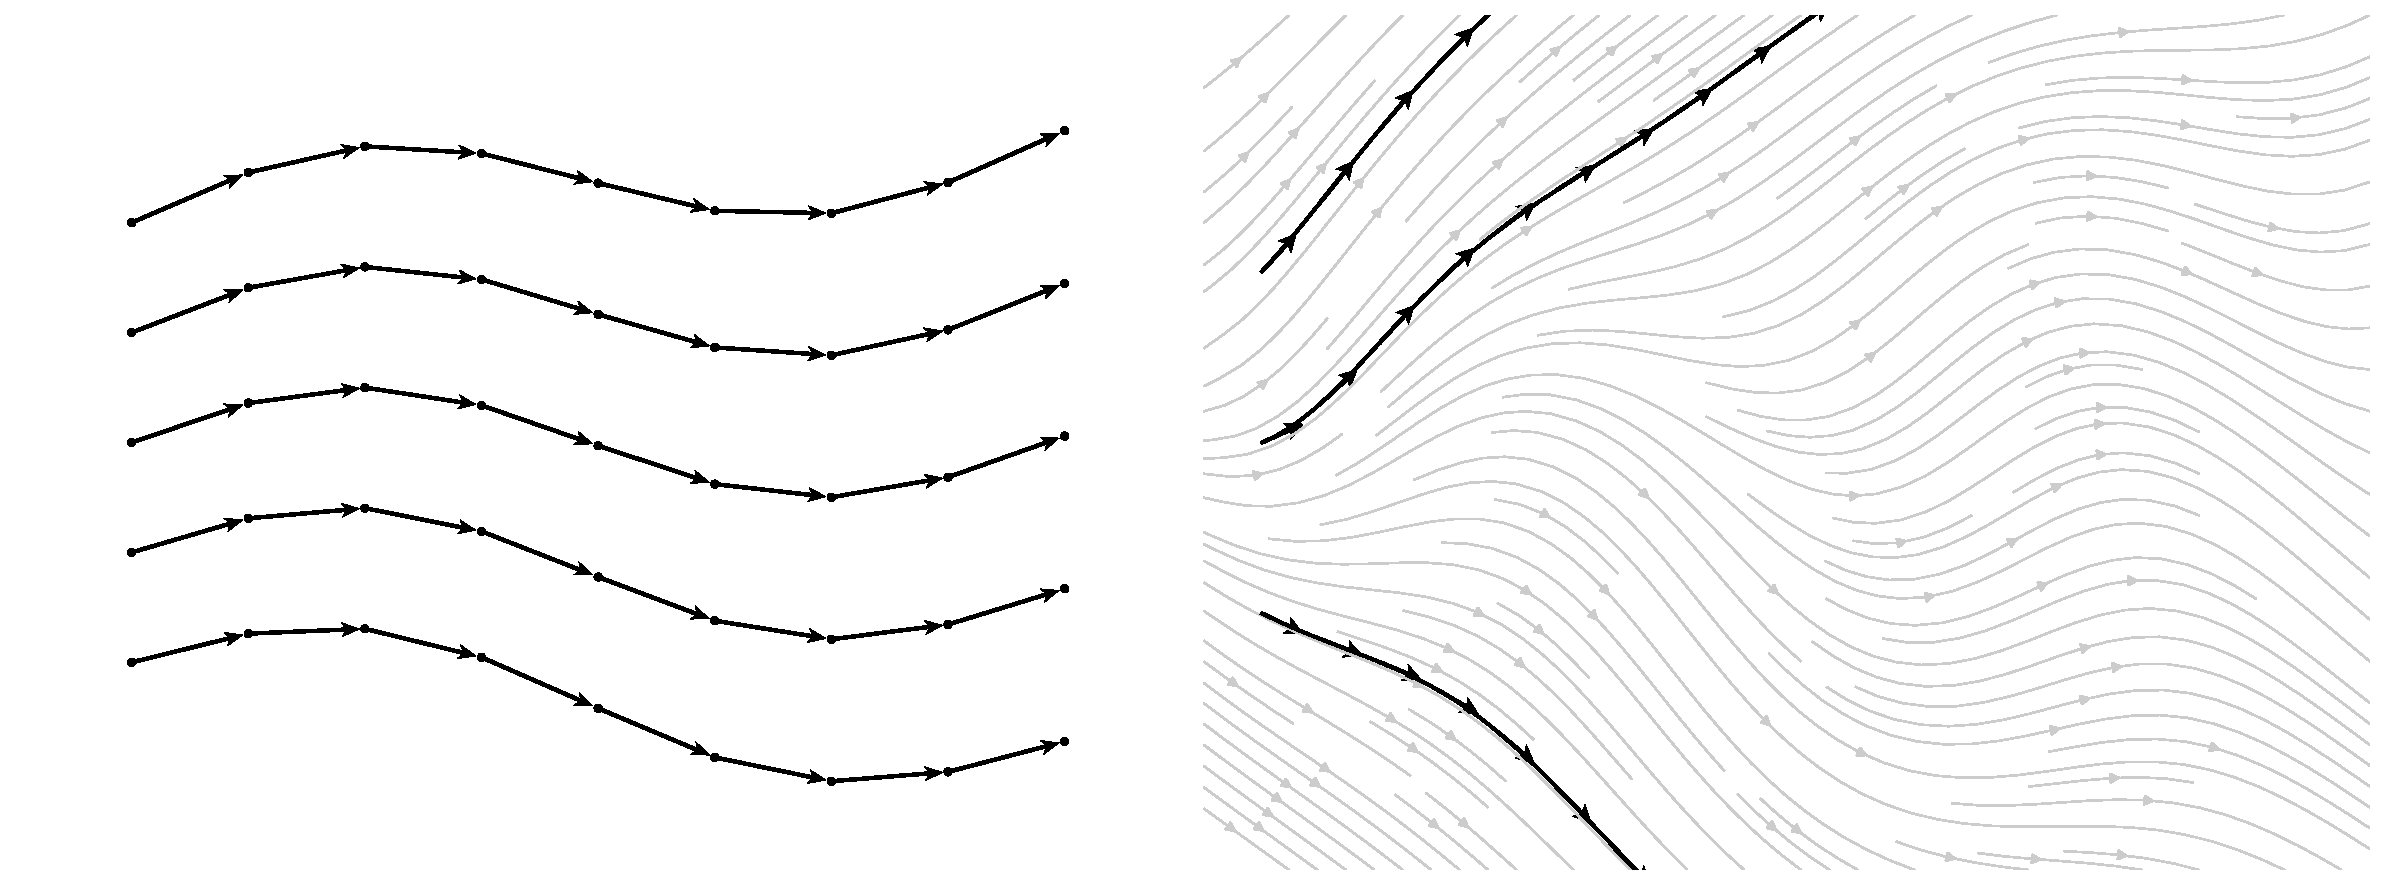
\includegraphics[width=\linewidth]{Images/PartE/discrete_vs_continuous_ode.pdf}
    \caption{\textbfs{ODE 插图。}
速度场 $\rvv(\rvx,t)$ 在每个点分配一个漂移矢量。
解轨迹 $\rvx(t)$ 是一条切线始终与局部漂移匹配的路径。
左侧面板显示了近似路径的逐步解算器更新（点和箭头），
而右侧面板显示与速度场一致的精确轨迹（黑色）。在不指定初始状态 $\rvx(0)$ 的情况下，存在无限多个其瞬时变化与相同速度场匹配的轨迹。
然而，一旦 $\rvx(0)$ 被固定，ODE 就会确定根据漂移流动的唯一路径 $\rvx(t)$。
\figcredit{由作者创建。}}
    \label{fig:ode-illustration}
\end{figure}

为了建立直觉，请将向量场 $\mathbf{v}(\mathbf{x}, t)$ 想象为一个动态的箭头景观，它告诉您点 $\mathbf{x}$ 在任何给定时间 $t$ 应该如何移动。求解微分方程意味着通过该场绘制一条曲线 $\mathbf{x}(t)$，使得该曲线在任意点的切线（即瞬时速度）与 $\mathbf{v}(\mathbf{x}(t), t)$ 给出的矢量对齐。
\begin{itemize}
    \item \textbfs{矢量场透视：} 函数 $\mathbf{v}(\mathbf{x}, t)$ 定义物体应如何移动：它给出运动或变化的局部“指令”。
    \item \textbfs{轨迹透视：} 解$\mathbf{x}(t)$是粒子在每一时刻遵守矢量场$\mathbf{v}$设定的规则时将遵循的路径。
\end{itemize}
因此，求解 ODE 就像将一个粒子放入流场中并观察它随时间的变化。

\subsection{常微分方程的存在唯一性}
到目前为止，我们已经看到，求解 ODE 意味着找到一条遵循向量场在每个点给出的方向的路径。直观上，这就像跟踪粒子沿着由速度定义的流移动时的轨迹。

但这张图引出了一个重要的问题：
\begin{question}
    如果我们选择一个起点，我们能否确定确实存在一条遵循这些方向的路径？如果存在，那条路径是唯一的，还是粒子会突然跳到不同的轨道上？
\end{question}

要从初始位置可靠地预测系统的行为，就要知道从那里出发的轨迹是否存在、是否唯一。\emph{存在唯一性定理}给出了向量场应满足的条件，是 ODE 理论的基础。


\paragraph{局部（时间）存在唯一性定理。}


给定初始条件，下面的局部定理保证解在初始时刻的某个邻域内存在且唯一。

\thmp{局部存在唯一性定理}{ode-local}{
设 $\mathbf{v}(\mathbf{x}, t)$ 在区域 $D \subseteq \mathbb{R}^D \times \mathbb{R}$ 上关于 $\mathbf{x}$ 和 $t$ 连续，并且关于 $\mathbf{x}$ 满足利普希茨条件
\[
\|\mathbf{v}(\mathbf{x}_1, t) - \mathbf{v}(\mathbf{x}_2, t)\| \leq L \|\mathbf{x}_1 - \mathbf{x}_2\| \quad \forall (\mathbf{x}_1, t), (\mathbf{x}_2, t) \in D,
\]
其中 $L > 0$ 为常数。那么，对每个初始条件 $\mathbf{x}(t_0) = \mathbf{x}_0$，\Cref{eq:general_ode} 在某个区间 $[t_0 - \delta, t_0 + \delta]$ 上存在唯一解 $\mathbf{x}(t)$。}{（证明概要）用 Picard--Lindel\"of 迭代可以构造性地证明该定理。以下迭代生成的函数列 $\{\mathbf{x}_n(t)\}$ 收敛到解 $\mathbf{x}(t)$。
\[
\mathbf{x}_{n+1}(t) = \mathbf{x}_0 + \int_{t_0}^t \mathbf{v}(\mathbf{x}_n(s), s) \diff s.
\]
\begin{itemize}
    \item 取初始近似 $\mathbf{x}_0(t) = \mathbf{x}_0$。
    \item 按上述积分公式逐次更新 $\mathbf{x}_n(t)$。
    \item 在利普希茨条件下，用巴拿赫不动点定理可证明迭代收敛。
\end{itemize}
}
\Cref{sec:picard} 还利用这一迭代思想加速扩散模型采样。


\paragraph{全局（时间）存在唯一性定理。}
加上适当的正则性条件，解的存在唯一性可以从初始时刻附近扩展到整个区间 $[t_0, T]$。\emph{卡拉泰奥多里定理}给出了这样一组条件，其中两项关键假设是关于状态变量的局部利普希茨连续性和线性增长界。
\begin{enumerate}[label=(\roman*)]
    \item \textbfs{关于 $\mathbf{x}$ 的局部利普希茨条件。} 存在 $[0, T]$ 上可积的函数 $\mathrm{Lip}(t)$，使得对任意 $\mathbf{x}_1, \mathbf{x}_2 \in \mathbb{R}^D$ 均有
    \[
    \|\rvv(\mathbf{x}_1, t) - \rvv(\mathbf{x}_2, t)\| \leq \mathrm{Lip}(t) \|\mathbf{x}_1 - \mathbf{x}_2\|.
    \]

    \item \textbfs{线性增长条件。} 存在 $[0, T]$ 上可积的函数 $M(t)$，使得对任意 $\mathbf{x} \in \mathbb{R}^D$ 均有
    \[
    \|\rvv(\mathbf{x}, t)\| \leq M(t)(1 + \|\mathbf{x}\|).
    \]
\end{enumerate}
我们建议读者参考 \citep{reid1971ordinary} 来全面讨论该定理的假设、形式陈述和详细证明。

\rmkb{为了将这些定理应用于扩散模型中的概率流 ODE（参见\Cref{eq:prob_ode_gt}），可能需要对分数函数$\nabla_\rvx \log p_t(\rvx)$施加额外的假设，例如条件（i）和（ii）。不关注技术细节的读者可以合理地接受这些假设，无需进一步论证。
}

总之，当给由时间相关的速度场定义的 ODE 指定一个初始条件后，粒子流的轨迹就被唯一确定了。

\paragraph{ 唯一性意味着解不相交} 由局部存在唯一性定理保证的 ODE 中解的唯一性意味着一个基本属性：从不同的初始条件开始的两个不同的解轨迹不能相互交叉。这反映了 ODE 的确定性本质，确保每个状态沿着独特的路径演化。下面的推论正式化了这个结果。


\corp{解的非交集}{
Consider two solutions $\rvx_1(t)$ and $\rvx_2(t)$ to the ODE
\[
\frac{\diff \rvx(t)}{\diff t} = \rvv\left(\rvx(t),t\right), \quad t \in [0,T].
\]
Suppose they have distinct initial values $\rvx_1(0) \neq \rvx_2(0)$. Then, these solutions do not intersect on $[0,T]$, i.e.,
\[
\rvx_1(t) \neq \rvx_2(t) \quad \text{for all } t \in [0,T].
\]
}{为了矛盾起见，假设存在一些$t^* \in (0,T]$使得
\[
\mathbf{x}_1(t^*) = \mathbf{x}_2(t^*).
\]
定义两个解第一次相遇的时间为
\[
t_0 := \inf \{ t \in [0,T]|\mathbf{x}_1(t) = \mathbf{x}_2(t) \}.
\]
由于 $\mathbf{x}_1(0) \neq \mathbf{x}_2(0)$ 和 $t^*$ 包含在该集合中，因此得出 $t_0 > 0$。通过 $\mathbf{x}_1$ 和 $\mathbf{x}_2$ 的连续性，我们有
\[
\mathbf{x}_1(t_0) = \mathbf{x}_2(t_0).
\]

考虑初值问题
\[
\frac{\mathrm{d}\mathbf{x}(t)}{\mathrm{d}t} = \mathbf{v}(\mathbf{x}(t), t), \quad \mathbf{x}(t_0) = \mathbf{x}_1(t_0).
\]
根据 ODE 的唯一性定理，$\mathbf{x}_1$ 和 $\mathbf{x}_2$ 必须在区间 $[t_0, T]$ 上重合。向后应用时间上的唯一性同样意味着两个解在 $[0, t_0]$ 上一致。
因此，解满足
\[
\mathbf{x}_1(t) = \mathbf{x}_2(t) \quad \text{for all } t \in [0, T],
\]
这与 $\mathbf{x}_1(0) \neq \mathbf{x}_2(0)$ 的假设相矛盾。因此，我们得出结论：
\[
\mathbf{x}_1(t) \neq \mathbf{x}_2(t) \quad \text{for all } t \in [0, T].
\]

}

通过保证解路径不相交，该定理为流映射模型提供了隐蔽但至关重要的支撑（参见 \Cref{ch:distillation,ch:fast-scratch}）。


\subsection{指数积分因子}\label{app:exp-int-factor}
即使由一般时变速度 $\rvv$ 确定的 ODE 也不承认闭式解，在某些特殊情况下，我们可以解析地求解它们，或者通过将其公式简化为更好的结构公式来求解。
\paragraph{示例.}
考虑以下线性标量 ODE：
\[
\frac{\diff \rvx(t)}{\diff t} = L(t)\rvx(t),
\]
其中 $L(t) \in \mathbb{R}$ 是连续函数。该方程以封闭形式可解，并且其解是众所周知的（对于任何 $s$ 和 $t$）：
\[
\rvx(t) = \rvx(s) \cdot \exp\left( \int_s^t L(\tau) \,\diff \tau \right).
\]
此公式演示了解如何根据指数因子演化，该指数因子累积瞬态系数 $L(t)$ 的影响。这促使使用 \emph{ 指数积分因子 }：
\begin{align}\label{eq:exp-int-factor}
    \mathcal{E}(s \shortrightarrow t) := \exp\left( \int_s^t L(\tau)\diff \tau \right),
\end{align}
特别是在更一般的设置中，动态包括线性和非线性分量。


\paragraph{半线性 ODE 和指数积分因子.}
我们现在考虑一类更广泛的 ODE，称为 \emph{semi线性} ODE。这些方程将动力学分为线性部分（在状态变量中）和非线性余数：
\begin{align}\label{eq:semilinear-ode}
    \frac{\diff \rvx(t)}{\diff t} = L(t)\rvx(t) + \rmN(\rvx(t), t),
\end{align}
其中 $\rvx(t) \in \mathbb{R}^D$ 是状态向量，$L(t)$ 是标量值连续函数，$\rmN: \mathbb{R}^D \times [0,T] \to \mathbb{R}^D$ 是非线性向量场。这种半线性结构自然出现在许多物理和工程系统中。特别是，它还出现在扩散模型的概率流 ODE 公式中（参见 \Cref{eq:prob_ode_gt}）。认识到这种结构可以实现积分因子表示
分析处理已知的线性动力学，并将剩余项留给进行数值近似。这一原则在
\Cref{ch:solvers} 中研究的扩散 ODE 求解器。


\subparagraph{步骤 1：通过积分因子隔离非线性项。}
观察到我们可以通过从 \Cref{eq:semilinear-ode} 中的半线性 ODE 中减去线性漂移来隔离非线性部分：
\[
\frac{\diff \rvx(t)}{\diff t} - L(t)\rvx(t) = \rmN(\rvx(t), t).
\]
为了吸收线性项，我们将两边乘以逆积分因子：
\[
\mathcal{E}^{-1}(s \shortrightarrow t) = \exp\left(-\int_s^t L(\tau)\diff \tau \right).
\]
现在将乘积规则应用到左侧：
\begin{align*}
\mathcal{E}^{-1}(s \shortrightarrow t) \left( \frac{\diff \rvx(t)}{\diff t} - L(t)\rvx(t) \right)
&= \frac{\diff}{\diff t} \left[ \mathcal{E}^{-1}(s \shortrightarrow t) \rvx(t) \right].
\end{align*}
因此，等式变为：
\[
\frac{\diff}{\diff t} \left[ \mathcal{E}^{-1}(s \shortrightarrow t) \rvx(t) \right]
= \mathcal{E}^{-1}(s \shortrightarrow t) \rmN(\rvx(t), t).
\]

这种变换通过隔离非线性分量来简化原始方程，使我们能够完全关注变换后的坐标系中的非线性动力学。

\subparagraph{第 2 步：随时间积分。}
我们现在将$s$两侧整合到$t$：
\[
\int_s^t \frac{\diff}{\diff \tau} \left[ \mathcal{E}^{-1}(s \shortrightarrow \tau) \rvx(\tau) \right] \diff \tau
= \int_s^t \mathcal{E}^{-1}(s \shortrightarrow \tau) \rmN(\rvx(\tau), \tau)\diff \tau.
\]
左侧只是在 $t$ 和 $s$ 处计算的转换变量的差异：
\[
\mathcal{E}^{-1}(s \shortrightarrow t) \rvx(t) - \rvx(s).
\]
因此，我们得到：
\[
\mathcal{E}^{-1}(s \shortrightarrow t) \rvx(t)
= \rvx(s) + \int_s^t \mathcal{E}^{-1}(s \shortrightarrow \tau) \rmN(\rvx(\tau), \tau)\diff \tau.
\]

\subparagraph{第 3 步：求解 $\rvx(t)$.}
两边乘以指数流 $\mathcal{E}(s \shortrightarrow t)$ 得出解：
\begin{align}\label{eq:exp-int-factor-integration}
    \rvx(t) = \underbrace{\mathcal{E}(s \shortrightarrow t)  \rvx(s)}_{\text{linear part}} + \underbrace{\int_s^t \mathcal{E}(\tau \shortrightarrow t) \rmN(\rvx(\tau), \tau)\diff \tau}_{\text{nonlinear part}} .
\end{align}该解自然地分为线性和非线性分量。指数积分器通过以精确闭形式求解线性部分并仅离散化非线性残差来利用这种结构。这确保了步长由非线性动力学决定，而不是由潜在的大线性系数决定（例如，参见 \Cref{sec:prologue-solvers} 中指数欧拉更新和普通欧拉更新之间的比较）。


\subsection{常微分方程数值求解器}
\label{app:de-solver}

我们考虑 \Cref{eq:general_ode} 中的 ODE，
\[
\frac{\diff\mathbf{x}(t)}{\diff t}
=
\mathbf{v}(\mathbf{x}(t),t),
\]
连同初始条件。求解 ODE 意味着找到连续轨迹 $\mathbf{x}(t)$ 其瞬时变化符合各时刻的速度场$\mathbf{v}$。

等价地，解满足积分方程
\begin{equation}
\label{eq:integral_form}
\mathbf{x}(t)
=
\mathbf{x}(0)
+
\int_0^t
\mathbf{v}(\mathbf{x}(\tau),\tau)\diff\tau.
\end{equation}
如果这个积分不能以封闭形式计算，我们近似通过评估有限多个速度场来计算轨迹点。

\paragraph{从连续轨迹到数值更新。}
数值求解器首先选择离散时间网格
\[
t_0,t_1,\ldots,t_M
\]
并产生相应的近似值
\[
\mathbf{x}_0,\mathbf{x}_1,\ldots,\mathbf{x}_M
\]
到连续的轨迹。

差距
\[
h_i:=t_{i+1}-t_i
\]
是 \emph{ 步长 }。较小的台阶通常提供更多的本地化
有关轨迹的信息，但需要更多的功能评估。
因此，数值求解器的目的是使用可用的有效地评估$\mathbf{v}$，以便可以得到准确的轨迹通过相对较少的步骤获得。

不同的求解器主要在 \emph{ 中有所不同，其中用于求解的信息
下一次更新来自}。这导致了以下有用的组织。

\paragraph{A 数值求解器的结构视图.}
对于与本书相关的方法，区分两个广泛的方法是有用的数值观点。

\begin{itemize}
    \item \textbfs{时间步进方法：}
    从当前状态开始，求解器将轨迹从一个时间指向下一个时间。欧拉、龙格——库塔和亚当斯——巴什福斯方法是具有代表性的例子。

    在时间步进方法中，我们进一步区分：
    \begin{itemize}
        \item a \emph{单步法}，构造下一个状态
        根据当前状态和生成的任何其他评估在当前间隔内；和

        \item 和 \emph{ 多步方法 }，另外重用
        来自先前已完成步骤的信息。
    \end{itemize}

    \item \textbfs{并行时间观点：}
    与其严格地一个接一个地完成所有时间点，不如制定轨迹计算，以便在几个时间可以一起更新。定点结构，例如 Picard
    迭代为这个想法提供了基本机制。
\end{itemize}单步方法不应与单步方法混淆。
\emph{功能评估}。例如，欧拉使用一种速度评估
每一步，而龙格-库塔方法可以评估速度
次在中间 \emph{stages}，同时仍然是单步方法。
决定性的区别是来自先前完成的步骤的信息是否是必需的。

\msgu{心理图片}{}{
稍后用于扩散采样的数值 ODE 求解器思想可以组织如下：
\begin{align}\label{eq:classic-solvers}
    \begin{array}{c}
\begin{array}{rcl}
\text{\textbfs{Time-stepping}}
&\rightarrow&
\begin{cases}
\text{single-step: }
    & \text{Euler, Runge--Kutta},\\
\text{multistep}
    & \text{Adams--Bashforth},
\end{cases}
\\[12pt]
\text{\textbfs{Parallel-in-time}}
&\rightarrow&
\text{Picard fixed-point iteration}.
\end{array}
\\[6pt]
\downarrow
\\[-2pt]
\text{The same numerical ideas can be applied forward or backward in time.}
\end{array}
\end{align}
}

这种区别在后面的扩散采样中特别有用：
Runge--Kutta 型结构通过观察获得更丰富的信息
\emph{在}中是当前步骤，而 Adams--Bashforth 类型的结构
通过查看 \emph{backward} 先前计算的值来获取它。

\paragraph{求解正向和反向时间的常微分方程。}
上述分类法不依赖于 ODE 的方向集成的。在普通的前向积分中，
\[
t_{n+1}>t_n,
\qquad
h_n=t_{n+1}-t_n>0.
\]
相反，扩散采样通常从嘈杂的终端状态开始，
使用递减的时间网格，
\[
t_{n+1}<t_n,
\qquad
h_n=t_{n+1}-t_n<0.
\]

当步长为视为有符号数量。因此，ODE 的逆时积分确实不需要新的数值求解器系列；欧拉、龙格--库塔、
多步和相关方法都可以应用于递减时间网格。

这种简单的反转应该与反转 SDE 区分开来，其中随机动力学需要额外的分析。我们讨论这个问题在下一节中。


\subsection{代表性数值求解器}
\label{app:de-solver-examples}

上面的分类告诉我们求解器从哪里获取其下一步的信息更新。现在我们通过一些有代表性的人将这些想法具体化例子。

我们刻意保持清单简短。欧拉举例说明了最简单的单步更新；龙格--库塔方法说明了附加的使用当前步骤内的阶段；亚当斯--巴什福斯阐释了对过去的重用历史；皮卡迭代说明了背后的定点观点时间并行方法。

在下面的示例中，让
\[
t_{n+1}=t_n+h.
\]
步长 $h$ 的签名为：$h>0$ 用于前向积分，$h<0$ 用于反向整合。


\paragraph{Euler 法.}
欧拉方法是最简单的单步方法。它仅使用速度在当前间隔的开始处：
\[
\mathbf{x}_{n+1}
=
\mathbf{x}_n
+
h\,\mathbf{v}(\mathbf{x}_n,t_n).
\]
从几何角度来看，欧拉观察当前的运动方向并遵循一个完整的步骤的方向。

在标准平滑假设下，欧拉存在局部截断误差
$\mathcal O(h^2)$ 和全局错误 $\mathcal O(h)$。它的简单性使它一个有用的一阶基线，但当速度在一步中发生显着变化。\paragraph{Runge--库塔方法.}
欧拉仅使用间隔开始时的速度。龙格--库塔
（RK）方法通过评估额外的速度来获取更多信息
在同一步骤中生成 \emph{stages}。

因此，它们是 \emph{ 单步、多阶段 } 方法：所有信息
用于构造$\mathbf{x}_{n+1}$是从当前开始生成的点 $\mathbf{x}_n$，但一个步骤可能包含多个函数评估。

我们使用两种二阶方法来说明基本 RK 原理。

\subparagraph{显式中点法.}
显式中点法首先使用当前速度来预测间隔中途状态：
\[
\mathbf{x}_{\mathrm{mid}}
=
\mathbf{x}_n
+
\frac{h}{2}
\mathbf{v}(\mathbf{x}_n,t_n).
\]
然后，它评估该预测中点的速度并使用该速度完整更新的方向：
\[
\mathbf{x}_{n+1}
=
\mathbf{x}_n
+
h\,
\mathbf{v}
\left(
\mathbf{x}_{\mathrm{mid}},
t_n+\frac{h}{2}
\right).
\]

因此，不要假设起始速度仍然具有代表性在整个区间内，中点方法“查看”步骤内部在决定如何完成之前。


\subparagraph{Heun 方法（改进欧拉）.}
Heun 方法是另一种两阶段二阶龙格方法——库塔方法。
它不看中点，而是首先使用欧拉方法进行预测端点：
\[
\mathbf{x}_{\mathrm{pred}}
=
\mathbf{x}_n
+
h\,\mathbf{v}(\mathbf{x}_n,t_n).
\]
然后，它评估该预测端点处的速度并对起始速度和预测结束速度：
\[
\mathbf{x}_{n+1}
=
\mathbf{x}_n
+
\frac{h}{2}
\left[
\mathbf{v}(\mathbf{x}_n,t_n)
+
\mathbf{v}(\mathbf{x}_{\mathrm{pred}},t_n+h)
\right].
\]

显式中点方法和 Heun 方法都使用两个阶段，并且在标准平滑假设，有局部截断误差
$\mathcal O(h^3)$ 和全局错误 $\mathcal O(h^2)$。它们的区别仅在于如何收集和组合额外的步骤内信息。

高阶龙格 - 库塔方法通过使用更多来扩展相同的原理阶段；此处省略其标准公式。在扩散采样中，
\citet{karras2022elucidating} 直接使用 Heun 方法作为 ODE 求解器。


\paragraph{Adams--巴什福斯方法.}
Runge--Kutta 方法通过查看获得附加信息
\emph{在}当前步骤内。相反，多步骤方法看起来
\emph{backward} 并重用之前完成的步骤中的信息。

例如，采用统一步长 $h$，二阶
Adams--Bashforth 方法 (AB2) 是
\[
\mathbf{x}_{n+1}
=
\mathbf{x}_n
+
h
\left[
\frac{3}{2}
\mathbf{v}(\mathbf{x}_n,t_n)
-
\frac{1}{2}
\mathbf{v}(\mathbf{x}_{n-1},t_{n-1})
\right].
\]
因此，第二条信息是存储的速度前一步而不是当前间隔内的新评估。

在标准平滑度假设和足够准确的情况下初始化，AB2 有局部截断错误$\mathcal O(h^3)$和全局错误 $\mathcal O(h^2)$。因为第一步没有历史记录，
多步方法必须首先使用另一个求解器进行初始化。

上面的公式假设网格是均匀的。在非均匀网格上，
多步系数取决于相邻步长。这个历史重用原则稍后将在特定扩散中再次出现多步求解器
\Cref{sec:exponential,subsec:dpm-solver++-multi}。\paragraph{皮卡迭代。}
上述方法通过构造局部轨迹来近似轨迹时间步进更新。皮卡迭代遵循不同的想法：
通过积分形式反复细化整个候选轨迹的常微分方程。

从最初的猜测开始
$\mathbf{x}^{(0)}(t)$ 满足
$\mathbf{x}^{(0)}(0)=\mathbf{x}(0)$，皮卡迭代定义
\[
\mathbf{x}^{(k+1)}(t)
=
\mathbf{x}(0)
+
\int_0^t
\mathbf{v}
\bigl(
\mathbf{x}^{(k)}(s),s
\bigr)
\diff s.
\]
每次迭代都沿上一条候选轨迹计算速度，再用这些速度构造新的轨迹。

这一迭代的不动点满足原 ODE 的积分方程。在 Picard--Lindel\"of 定理的标准条件下，迭代在局部收敛到 ODE 的解。

一次皮卡迭代中，各个时刻的速度只取决于\emph{上一条}候选轨迹，因此可以在时间维度上并行计算。\Cref{sec:picard} 会用到这个性质。


\section{随机微分方程基础}\label{app:sde-intro}

随机微分方程 (SDE) 是常微分方程 (ODE) 的扩展，它包含随机性，为受不确定性影响的系统建模提供了数学框架。本章介绍 SDE，从 ODE 的离散化开始，扩展到 SDE 的离散化，最后讨论一般的 SDE，包括伊藤微积分和伊藤公式。

\subsection{从 ODE 到 SDE：直观介绍}
让我们从描述状态变量 $ \rvx(t) \in \mathbb{R}^D $ 的确定性演化的 ODE 开始：
\begin{equation}
    \frac{\diff\rvx(t)}{\diff t} = \rvf(\rvx(t), t), \quad \rvx(0) = \rvx_0.
    \label{eq:ode}
\end{equation}
此处，$ \rvf: \mathbb{R}^D \times [0,T] \rightarrow \mathbb{R}^D $ 是一个与时间相关的速度场，控制 $ \rvx(t) $ 的动力学。该 ODE 的解是一条平滑轨迹 $ t \mapsto \rvx(t) $，完全由初始条件 $ \rvx_0 $ 确定。

\paragraph{离散化透视.} 为了建立直觉，请考虑 \Cref{eq:ode} 在小时间步长 $ \Delta t $ 上的欧拉离散化：
\begin{equation*}
    \rvx_{t+\Delta t} = \rvx_t + \rvf(\rvx_t, t) \Delta t.
\end{equation*}
当 $ \Delta t \to 0 $ 时，这种近似变得更加准确，收敛（在 $ \rvf $ 上的标准正则条件下）到 ODE 的精确解。\paragraph{随机性介绍：从 ODE 到 SDE。} 在许多现实系统中，完美的动力学知识是不现实的。噪声、不确定性或未建模的相互作用可能会影响进化。为了纳入这种随机性，我们用随机项增强 ODE：
\begin{equation}
    \rvx_{t+\Delta t} = \rvx_t + \rvf(\rvx_t, t)\Delta t + g(t)\sqrt{\Delta t} \cdot \bm{\epsilon}_t,
    \label{eq:euler-sde}
\end{equation}
其中
\begin{itemize}
    \item $g: [0,T] \to \mathbb{R}$ 是扩散系数（可能取决于状态和时间，尽管这里假设仅取决于时间），
    \item $\bm{\epsilon}_t \sim \mathcal{N}(\bm{0}, \rmI_D)$ 是独立同分布的标准高斯向量。
\end{itemize}

此修改后的更新规则不仅反映了确定性漂移，还反映了按 $ \sqrt{\Delta t} $ 缩放的随机扰动。缩放确保随机扰动在极限 $ \Delta t \to 0 $ 内保持有限。重要的是，这个公式产生了 \emph{ 连续时间随机过程 } 作为 $ \Delta t \to 0 $，这将我们引向 SDE 的框架。

\paragraph{随机微分方程.}
形式上，离散更新 ~\Cref{eq:euler-sde} 的限制为 $ \Delta t \to 0 $ 定义 SDE：
\begin{equation}
    \diff \rvx(t) = \rvf(\rvx(t), t)\diff t + g(t) \diff \rvw(t).
    \label{eq:sde}
\end{equation}
这里，$ \rvw(t) \in \mathbb{R}^D $是一个\emph{维纳过程}（标准布朗运动），一个连续时间随机过程，其特征在于：
\begin{itemize}
    \item \textbfs{初始状态：} $ \rvw(0) = 0 $ 几乎肯定；
    \item \textbfs{独立增量：}为$ 0 \leq s < t $，增量$ \rvw(t) - \rvw(s) $与过去无关；
    \item \textbfs{高斯增量：}
    \begin{align}\label{eq:wiener-gaussian}
        \rvw(t) - \rvw(s) \sim \mathcal{N}\bigl(\bm{0}, (t - s)\rmI_D \bigr)
    \end{align}
    \item \textbfs{连续性：} 样本路径 $ t \mapsto \rvw(t) $ 几乎肯定是连续的，但不可微分。
\end{itemize}
此外，符号
\[
\diff \rvw(t) := \rvw(t + \diff t) - \rvw(t)
\]
通常用来表示维纳过程的无穷小增量。

虽然具有启发性，但这种表示法是启发式的，不应被解释为经典微分（例如，在黎曼或勒贝格意义上），因为布朗路径几乎肯定是不可微分的。相反，它作为表达高斯增量属性的正式简写：
\[
\diff \rvw(t) \sim \mathcal{N}(0, \diff t\, \mathrm{I}_D),
\]
这意味着在长度 $ \diff t $ 的无穷小时间间隔内，维纳过程的增量表现得像均值和协方差为零的高斯随机变量 $ \diff t\, \mathrm{I}_D $。


\subsection{关于 \Cref{eq:sde} 的进一步说明}
\Cref{eq:sde} 中的 SDE 应按其\emph{积分形式}理解。
\begin{align}\label{eq:sde-integral-form}
    \rvx(t) = \rvx(0) + \int_0^t \rvf(\rvx(s), s) \diff s + \int_0^t g(s) \diff \rvw(s),
\end{align}
解释为 \emph{Itô 意义 }。
这里，第一项是代表累积确定性漂移的经典（黎曼或勒贝格）积分，而第二项是 \emph{伊藤随机积分}，它相对于维纳过程 $ \rvw(t) $ 进行积分。我们不提供伊藤积分的完整严格构造，但提供以下直觉。\paragraph{伊藤积分的直观理解。}
It\^o 积分可以理解为离散和的极限
形式 \footnote{ 对于平方可积被积函数，这种收敛在 $L^2$ 意义上（均方）成立，这又意味着概率收敛。 $L^2$ 观点是自然的，因为它直接连接到 It\^o 的等距，这是 It\^o 积分的标准和严格构造的关键恒等式。该等距将随机积分与期望的标准积分（$\E\bigl[\bigl\|\int_0^T \bm{\psi}(t)\,\mathrm{d}\rvw_t \bigr\|^2\bigr] = \E\bigl[\int_0^T \|\bm{\psi}(t)\|_F^2\,\mathrm{d}t\bigr]$ 与 Frobenius 范数）联系起来
$\|\bm{\psi}(t)\|_F^2$）；我们在 \Cref{subsec:rigorous-proof-linear-sde}.} 中声明并使用它
\[
\sum_i g(t_i)\bigl(w(t_{i+1})-w(t_i)\bigr),
\]
其中被积函数 $g(t)$ 在 \emph{left} 端点处计算
每个子区间的 $t_i$。随着分区变得更精细，这些总和收敛到 It\^o 积分。左点评价规则是将 It\^o 积分与经典积分区分开来，后者可以使用中点或其他评估规则。因为布朗路径是连续但几乎肯定无处可微，经典积分并不直接适用。 It\^o 积分可以处理这个问题不规则性并捕获随机的累积效应随时间的波动。

\paragraph{微分表示法的使用.}
$ \diff \rvx(t) $、$ \diff t $ 和 $ \diff \rvw(t) $ 等表达式不是经典微分。相反，它们是表示各个过程的无限小的增量的正式符号。虽然是启发式的，但它们被广泛使用，因为它们可以方便地表达与 ODE 类似的 SDE，并促进伊藤演算中的正式操作。

\Cref{app:Ito} 中将解释 伊藤微积分如何应用于扩散模型。


\paragraph{与常微分方程的比较.}
在 ODE 中，例如
\[
\frac{\diff \rvx(t)}{\diff t} = \rvf(\rvx(t), t),
\]
积分形式
\[
\rvx(t) = \rvx(0) + \int_0^t \rvf(\rvx(\tau), \tau) \diff \tau
\]
由微积分 \emph{ 基本定理 } 证明，该定理确保可微函数可以从其导数中恢复。

相比之下，在 \Cref{eq:sde} 等 SDE 中，由于布朗运动缺乏可微性，并且随机积分不遵循经典链式法则，因此没有直接模拟该定理。相反，伊藤微积分引入了替代工具（例如伊藤引理）来分析和操纵随机动力学。

因此，虽然 SDE 的微分表示法紧凑且直观，但严格的理解取决于使用 Itô 积分通过积分公式来解释它们。

\subsection{SDE 的数值求解器}

与 ODE 一样，只要 $\mathbf{f}(\cdot, t)$ 与 $g(\cdot)$ 满足一定的光滑性条件，\Cref{eq:sde} 中的 SDE 就有唯一解\footnote{这里的解是\emph{强}意义下的解，即对固定的概率空间上给定的布朗运动 $\mathbf{w}(\cdot)$，$\mathbf{x}(t)$ 满足 SDE 的积分形式（见 \Cref{eq:sde-integral-form}）。详细的技术定义从略。}：$\mathbf{f}(\cdot, t)$ 关于 $\mathbf{x}$ 利普希茨且具有线性增长，$g(\cdot)$ 平方可积。

对于 \Cref{eq:sde} 这样的 SDE，一般情形下没有闭式解，因而必须借助数值方法。常用的一种是 \emph{欧拉—丸山法}，它推广了 ODE 的欧拉法，事实上我们在 \Cref{eq:euler-sde} 中已经见过它。该方法在一个时间步长 $\Delta t$ 上对漂移项 $\rvf(\rvx(t), t)$ 作近似，并用高斯增量 $\sqrt{\Delta t}\,\boldsymbol{\epsilon}_t$（其中 $\boldsymbol{\epsilon}_t \sim \mathcal{N}(\mathbf{0}, \mathbf{I})$）来模拟随机噪声 $g(t) \diff \rvw(t)$。

后文 \Cref{subsec:rigorous-proof-linear-sde} 会看到，线性 SDE 是有闭式解的。


